\documentclass[a4paper,10pt]{article}
\usepackage[latin1]{inputenc}
\usepackage[english]{babel}
\usepackage{amsmath}
\usepackage{amsfonts}
\usepackage{amssymb}
\usepackage{titling}
\usepackage{nomencl}
\usepackage{booktabs}
\usepackage{graphicx}
\usepackage[style=ieee,backend=bibtex]{biblatex}
\usepackage{fancyhdr}
\usepackage{varioref}
\usepackage[activate={true,nocompatibility},final,tracking=true,kerning=true,spacing=true,factor=1100,stretch=10,shrink=10]{microtype}
% activate={true,nocompatibility} - activate protrusion and expansion
% final - enable microtype; use "draft" to disable
% tracking=true, kerning=true, spacing=true - activate these techniques
% factor=1100 - add 10% to the protrusion amount (default is 1000)
% stretch=10, shrink=10 - reduce stretchability/shrinkability (default is 20/20)

% Reduce tracking around small caps to 40%
\SetTracking{encoding={*}, shape=sc}{40}

% Path to images.
\graphicspath{{img/}}

% Setup nomenclature.
\makenomenclature
\setlength{\nomitemsep}{-\parsep}

% Setup bibiliography.
\addbibresource{bibliography}

% Document info.
\author{Z0966990}
\title{Statistics Assignment}
\date{\today}

% Header and footer.
\pagestyle{fancy}
\fancyhf{}
\lhead{\thetitle}
\rhead{\theauthor}
\cfoot{\thepage}
\renewcommand{\headrulewidth}{0pt}
\renewcommand{\footrulewidth}{0pt}

\begin{document}
    
% Title page.
\begin{titlepage}
    \centering
    \vspace*{\fill}
    
\includegraphics[width=0.5\textwidth]{Durham}\\
    \vspace*{\fill}
    \LARGE\thetitle\\
    \large\theauthor\\
    \large L2 Engineering Mathematics\\
    \large\thedate\\
    \vspace*{\fill}
\end{titlepage}

% Nomenclature.
\nomenclature[0]{$n_{out}$}{Number of datapoints outside the 95\% confidence 
interval for the mean.}
\nomenclature[1]{$\bar{x}$}{Mean total energy consumption for sample.}
\printnomenclature

% Main matter.
\section{Introduction}

Statistical analysis was used to identify the demand patterns of energy 
consumption in a range of homes on a summer and winter's day.

In 2009 the Irish Commission for Energy Regulation (CER) undertook a trial 
where smart meters were installed in 6256 homes \cite{martinsmart}. Those 
meters recorded the rate  of electrical energy consumption every half hour for 
a year.

This report analysed the total energy consumption for two days in the 
trial---the first day which occurred in the summer and the 200th day which 
occurred in the winter. In order to get an idea for the total energy 
consumption for each day, the half hourly consumption rates were summed for 
each meter.

Furthermore, it was noted a large number of meters recorded no energy 
consumption. This could have been due to the consumers being away from the 
premises or the meters being faulty. These meters were excluded from 
statistical analysis to avoid skewing the mean of the distribution.

\section{Demand Patterns}

Figure~\vref{fig:Data} shows the distribution of the total energy consumption 
for 6122 smart meters on day 1 and day 200. The histograms do not include the 
meters which recorded no energy consumption that day.
    
\begin{figure}[h]
    \centering
    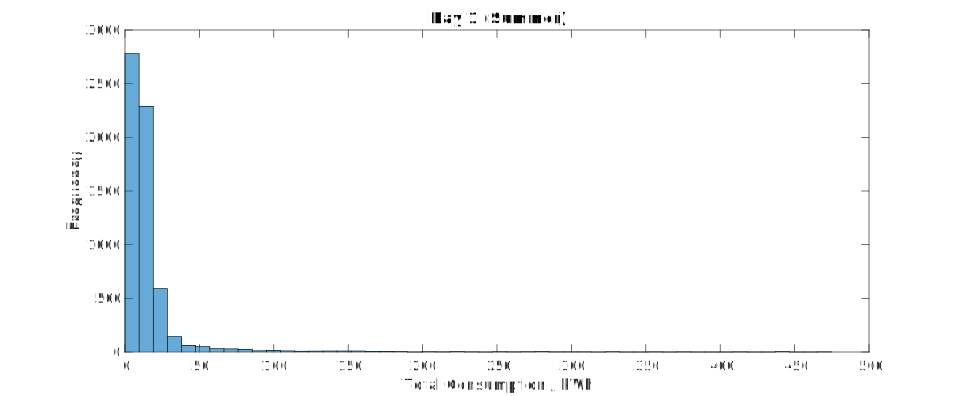
\includegraphics[width=0.48\textwidth]{Day1}
    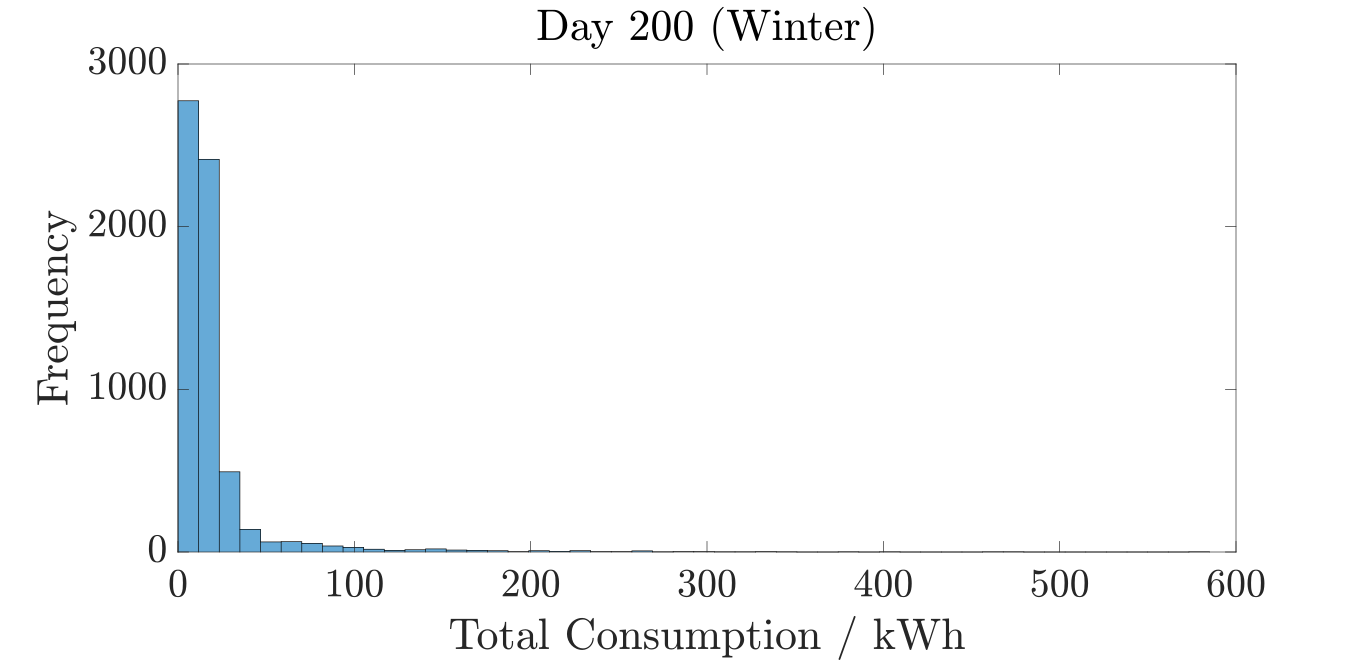
\includegraphics[width=0.48\textwidth]{Day200}
    \caption{Frequency histogram of total energy consumption on each day.}
    \label{fig:Data}
\end{figure}

From initial inspection, it was clear for both distributions the data had a 
strong negative skew with a large number of meters reporting total consumption 
under 100 and then outliers up to 1200. This made it difficult to discern 
details in the dataset when only 50 bins were used.

However, the 90\% and 95\% confidence intervals for the mean total consumption 
still yielded statistically significant results. Table~\vref{table:Mean} 
records the upper and lower bounds for the mean at two different confidence 
levels.

\begin{table}[h]
    \centering
    \begin{tabular}{llll}
        \toprule
        \textbf{Day} & $\bar{x}$ & 90\% Interval & 95\% Interval \\
        \midrule
        \textbf{Summer} & 31.265 & [30.608, 31.922] & [30.482, 32.048] \\
        \textbf{Winter} & 39.575 & [38.749, 40.402] & [38.591, 40.560] \\
        \bottomrule
    \end{tabular}
    \caption{Confidence intervals for mean energy consumption on each day.}
    \label{table:Mean}
\end{table}

The 90\% and 95\% confidence intervals for the population mean total energy 
consumption on each day did not overlap. The upper bound of the 95\% interval 
on the summer's day at 32.048 was less than the lower bound of the 95\% 
interval on the winter's day at 38.591. This suggests at the 5\% level of 
significance, the mean total energy consumption on day 200 in the winter for 
all Irish households was greater than on day 1 in the summer.

\section{Outliers}

In order to eliminate the outliers in the dataset and achieve a more 
symmetrical distribution, the data for day 1 was revised by 

\begin{figure}[h]
    \centering
    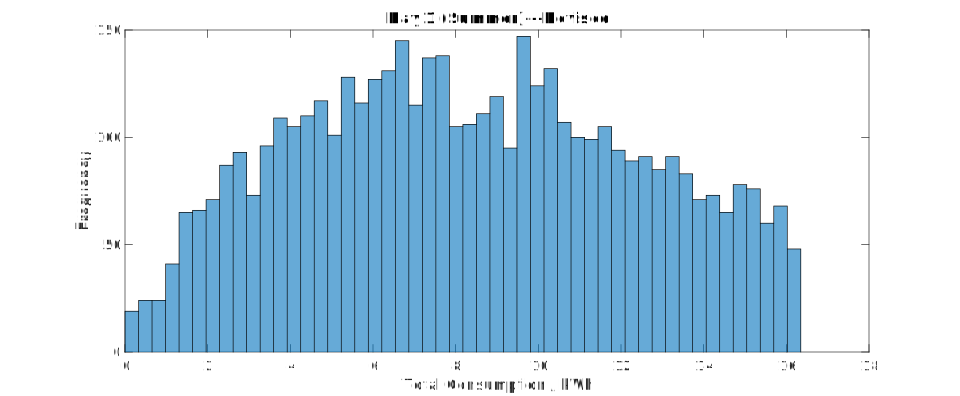
\includegraphics[width=0.48\textwidth]{Day1Revised}
    \caption{Frequency histogram of revised total energy consumption on day 1.}
    \label{fig:NoOutliers}
\end{figure}

\begin{table}[h]
    \centering
    \begin{tabular}{llll}
        \toprule
        \textbf{Data} & $\bar{x}$ & 95\% Interval & $n_{out}$ \\
        \midrule
        \textbf{Original} & 31.265 & [30.482, 32.048] & 3836 \\
        \textbf{Revised}  & 16.471 & [16.241, 16.701] & 4541 \\
        \bottomrule
    \end{tabular}
    \caption{Number of values outside the 95\% confidence interval for mean 
    total energy consumption on day 1.}
    \label{table:Outliers}
\end{table}

% References.
\printbibliography

\clearpage

\end{document}